\documentclass[
  aspectratio=169,
  10pt,
  t,
]{beamer}

\usepackage[english]{babel}
\usepackage[utf8]{inputenc}
\usepackage[T1]{fontenc}
\usepackage{csquotes}
\usepackage[backend=bibtex,style=authoryear,maxcitenames=2,maxbibnames=3]{biblatex}
\addbibresource{references.bib}
\usepackage{booktabs}
\usepackage{tikz}
\usetikzlibrary{arrows.meta,positioning}

% ---------------------------------------------------------------- theme
\makeatletter
% Same structure as the template, without another university's branding.
% If you have the mubeamer files, replace this block with:  \usetheme[workplace=...]{MU}
\usepackage[sfdefault,lining]{FiraSans}
\usepackage[scale=0.86]{FiraMono}
\definecolor{ink}{HTML}{1B2A41}      % structure, titles
\definecolor{muted}{HTML}{5F5E59}    % secondary text
\definecolor{rule}{HTML}{D9D6CF}     % hairlines
\definecolor{pipeA}{HTML}{A64B2C}    % Pipeline A (terracotta, as in the GUI)
\definecolor{pipeB}{HTML}{3A6676}    % Pipeline B (slate, as in the GUI)
\definecolor{accent}{HTML}{1D4ED8}   % \alert
\definecolor{good}{HTML}{2E6B3F}
\usetheme{default}
\usecolortheme[named=ink]{structure}
\setbeamercolor{normal text}{fg=ink!92!black,bg=white}
\setbeamercolor{alerted text}{fg=accent}
\setbeamercolor{frametitle}{fg=ink}
\setbeamercolor{framesubtitle}{fg=muted}
\setbeamercolor{block title}{fg=white,bg=ink}
\setbeamercolor{block body}{bg=ink!5}
\setbeamercolor{block title example}{fg=white,bg=good}
\setbeamercolor{block body example}{bg=good!7}
\setbeamercolor{block title alerted}{fg=white,bg=pipeA}
\setbeamercolor{block body alerted}{bg=pipeA!7}
\setbeamercolor{footline}{fg=muted}
\setbeamerfont{frametitle}{size=\large,series=\bfseries}
\setbeamerfont{framesubtitle}{size=\small,series=\mdseries}
\setbeamerfont{footline}{size=\scriptsize}
\setbeamerfont{caption}{size=\scriptsize}
\setbeamertemplate{navigation symbols}{}
\setbeamertemplate{itemize items}{\raisebox{0.15ex}{\scriptsize$\blacktriangleright$}}
\setbeamertemplate{itemize subitem}{\textendash}
\setbeamertemplate{enumerate items}[default]
\setbeamertemplate{blocks}[rounded]
\setbeamertemplate{caption}{\raggedright\insertcaption\par}
\setbeamertemplate{frametitle}{%
  \vskip0.7em
  \usebeamerfont{frametitle}\usebeamercolor[fg]{frametitle}\insertframetitle
  \ifx\insertframesubtitle\@empty\else
    \par\vskip0.15em{\usebeamerfont{framesubtitle}\usebeamercolor[fg]{framesubtitle}\insertframesubtitle}\fi
  \par\vskip0.3em{\color{rule}\rule{\textwidth}{0.6pt}}\vskip-0.2em}
\setbeamertemplate{footline}{%
  \leavevmode\hbox to\paperwidth{\hskip1.2em
    \usebeamerfont{footline}\usebeamercolor[fg]{footline}%
    \insertshorttitle\quad\textperiodcentered\quad\insertshortauthor\hfill
    \insertsectionhead\hfill\insertframenumber\,/\,\inserttotalframenumber\hskip1.2em}%
  \vskip0.9em}
\setbeamertemplate{title page}{%
  \vskip2.5em
  {\color{pipeA}\rule{2.2em}{3pt}}\par\vskip1em
  {\usebeamerfont{title}\usebeamercolor[fg]{title}\bfseries\LARGE\inserttitle\par}
  \vskip0.6em
  {\large\color{muted}\insertsubtitle\par}
  \vskip2.2em
  {\insertauthor\par}\vskip0.3em
  {\small\color{muted}\insertinstitute\par}\vskip0.3em
  {\small\color{muted}\insertdate\par}}
\setbeamertemplate{section page}{%
  \vfill{\color{pipeA}\rule{2.2em}{3pt}}\par\vskip0.8em
  {\Huge\bfseries\color{ink}\insertsectionhead\par}\vskip0.5em
  {\large\color{muted}\insertsubsectionhead\par}\vfill}
% Roadmap: the brief's six verbs, current step(s) highlighted. Usage: \roadmap{from}{to}{note}
\newcommand{\roadmap}[3]{%
\begin{frame}[c,plain,noframenumbering]
\centering
\begin{tikzpicture}[font=\large\bfseries]
  \foreach \w [count=\i] in {Select,Order,Implement,Compare,Evaluate,Justify} {
    \pgfmathtruncatemacro{\on}{and(\i>=#1,\i<=#2)}
    \ifnum\on=1 \def\c{pipeA}\else\def\c{ink!25}\fi
    \ifnum\i=1 \node[text=\c] (w\i) {\w};
    \else \pgfmathtruncatemacro{\p}{\i-1}\node[text=\c, right=6.5mm of w\p] (w\i) {\w};
      \draw[-{Stealth[length=1.6mm]}, ink!25, thick] ([xshift=1.5mm]w\p.east) -- ([xshift=-1.5mm]w\i.west); \fi
  }
\end{tikzpicture}
\par\vskip1.4em
{\color{muted}#3\par}
\end{frame}}
\setbeamersize{text margin left=7mm, text margin right=7mm}
\setlength{\leftmargini}{1.2em}
\setlength{\leftmarginii}{1.1em}
\newcommand{\A}{\textcolor{pipeA}{\textbf{A}}}
\newcommand{\B}{\textcolor{pipeB}{\textbf{B}}}
\newcommand{\pA}[1]{\textcolor{pipeA}{#1}}
\newcommand{\pB}[1]{\textcolor{pipeB}{#1}}
\newcommand{\muted}[1]{\textcolor{muted}{#1}}
\renewcommand{\arraystretch}{1.12}
\makeatother
% ---------------------------------------------------------------- end theme

\title[Video-Game Search Engine]{A Search Engine for Video-Game Knowledge}
\subtitle[Text Analysis \& Boolean Retrieval]{Text analysis, indexing and Boolean retrieval with two competing pipelines}
\author[Priyanka B, Sachin B, Tiya P, Vaidhav A]{Priyanka B \textperiodcentered\ Sachin B \textperiodcentered\ Tiya P \textperiodcentered\ Vaidhav A}
\institute[Vidyashilp University]{Course code DATA403: Natural Language Processing \textperiodcentered\ Assessment-1\texorpdfstring{\\}{, }Vidyashilp University, Bangalore}
\date{October 2026}
\subject{Domain-Specific Text Analysis and Retrieval System}
\keywords{NLP, information retrieval, inverted index, Boolean search, stemming, lemmatization}
\begin{document}

\begin{frame}[plain]
\maketitle
\end{frame}

% =====================================================================
\section{The Problem}

\begin{frame}{What we built}{A complete classical search engine, measured at every stage}
\begin{columns}[T]
\begin{column}{.47\textwidth}
\begin{itemize}
  \item \structure{Indexer} (ahead of time): reads every document, builds a lookup table of every term and where it occurs
  \item \structure{Searcher} (at question time): looks terms up, combines them with \texttt{AND} / \texttt{OR} / \texttt{NOT}, ranks the result
  \item Everything in between decides \alert{which ``words'' exist at all}
  \item Two pipelines make \alert{opposite bets} on that decision; we compare them under rules fixed in advance
\end{itemize}
\end{column}
\begin{column}{.5\textwidth}
\centering
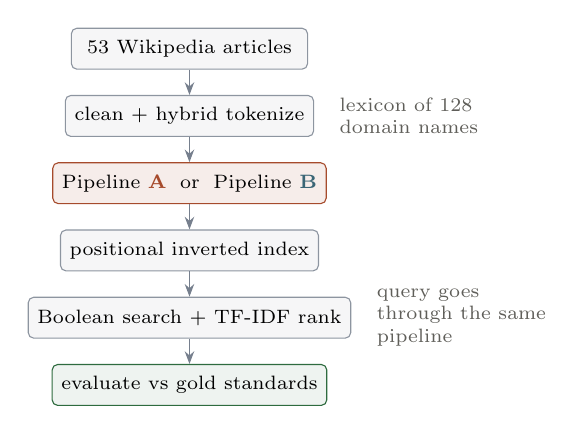
\begin{tikzpicture}[font=\scriptsize, node distance=3.2mm,
  box/.style={draw=ink!50, rounded corners=2pt, fill=ink!4, minimum width=30mm, minimum height=5.2mm, align=center},
  arr/.style={-{Stealth[length=1.6mm]}, ink!60}]
  \node[box] (d) {53 Wikipedia articles};
  \node[box, below=of d] (c) {clean + hybrid tokenize};
  \node[box, below=of c, fill=pipeA!10, draw=pipeA] (p) {Pipeline \A{} \;or\; Pipeline \B{}};
  \node[box, below=of p] (i) {positional inverted index};
  \node[box, below=of i] (s) {Boolean search + TF-IDF rank};
  \node[box, below=of s, fill=good!8, draw=good] (e) {evaluate vs gold standards};
  \foreach \a/\b in {d/c,c/p,p/i,i/s,s/e} \draw[arr] (\a) -- (\b);
  \node[right=2mm of c, text width=22mm, muted] {lexicon of 128 domain names};
  \node[right=2mm of s, text width=22mm, muted] {query goes through the same pipeline};
\end{tikzpicture}
\end{column}
\end{columns}
\end{frame}

\begin{frame}{Domain and data}{Why video games, and where the documents come from}
\begin{columns}[T]
\begin{column}{.5\textwidth}
\textbf{Hard for generic NLP tools}
\begin{itemize}
  \item hyphens and numbers in names: \emph{Counter-Strike}, \emph{Destiny 2}
  \item names made of everyday words: \emph{Tomb Raider}
  \item spelling variants: \emph{Game Boy / Gameboy}, \emph{SNES}
\end{itemize}
\vskip0.4em
\textbf{Corpus from MIRACL} \parencite{zhang2023miracl}
\begin{itemize}
  \item 12 real questions; their judged articles: relevant + \alert{hard negatives}
  \item full Wikipedia articles, \textbf{D01--D53}
\end{itemize}
\end{column}
\begin{column}{.46\textwidth}
\begin{table}
\small
\begin{tabular}{lr}
\toprule
Documents & 53 \\
Sentences & 9,305 \\
Tokens (hybrid) & 251,482 \\
Characters & 1,362,150 \\
Vocabulary (case-folded) & 16,030 \\
Avg.\ length (tokens) & 4,744.9 \\
\bottomrule
\end{tabular}
\caption{Corpus statistics (\texttt{corpus\_summary.csv})}
\end{table}
\muted{\scriptsize 53 $>$ 15--30 recommended: each question needs several relevant documents and some hard negatives, or precision and recall are meaningless.}
\end{column}
\end{columns}
\end{frame}

\begin{frame}{Gold standards: an answer key for every stage}
\begin{table}
\small
\begin{tabular}{p{.22\textwidth}p{.46\textwidth}p{.22\textwidth}}
\toprule
Gold standard & Contents & Evaluates \\
\midrule
Relevance judgments & 12 questions $\times$ 53 documents = 636 labels (57 relevant) & searcher, ranker \\
POS gold & 226 tokens, 8 corpus sentences, Penn Treebank & 5 POS taggers \\
NER gold & 51 entities, 7 types (PERSON \dots\ EVENT) & 2 entity recognisers \\
Domain lexicon & 128 names that must survive as one term & tokenizers, pipelines \\
Stemming groups & word families + a trap: \emph{universe} vs \emph{university} & stemmers, lemmatizers \\
\bottomrule
\end{tabular}
\end{table}
\begin{block}{Process discipline}
Hypotheses, metrics and the selection rule were \alert{preregistered before any result}; every later change is a dated amendment in the decision log.
Relevance labels: two reviewers under a written protocol, so search results are labelled \emph{preliminary}.
\end{block}
\end{frame}

% =====================================================================
\section{Select}
\roadmap{1}{1}{Choose each component by measuring it on the corpus}

\begin{frame}{Tokenization: where does a word end?}{The single most important choice}
\begin{columns}[T]
\begin{column}{.55\textwidth}
\begin{table}
\small
\begin{tabular}{lrrc}
\toprule
Tokenizer & Tokens & Term dict. & Names kept \\
\midrule
NLTK   & 253,416 & 16,619 & 0 / 91 \\
spaCy  & 261,849 & 15,745 & 0 / 91 \\
Custom (regex) & 252,750 & 16,664 & 0 / 91 \\
\textbf{Hybrid} & 251,482 & 16,030 & \alert{\textbf{91 / 91}} \\
\bottomrule
\end{tabular}
\caption{\texttt{tokenization\_comparison.csv}, \texttt{tokenizer\_domain\_terms.csv}}
\end{table}
\small
\texttt{Counter-Strike: Global Offensive}\\
\muted{spaCy:} \texttt{Counter | - | Strike | : | Global | Offensive}\\
\muted{hybrid:} \texttt{Counter-Strike\_Global\_Offensive}
\end{column}
\begin{column}{.42\textwidth}
\textbf{Hybrid} = custom regex rules + three domain steps:
\begin{enumerate}
  \item rewrite variants (\emph{Gameboy} $\rightarrow$ \emph{Game Boy})
  \item split lower-case compounds (\emph{first-person})
  \item merge lexicon names, longest first (\texttt{Game\_Boy})
\end{enumerate}
\vskip0.3em
Custom rules keep \emph{\$8.5}, \emph{U.S.}, \emph{PS4}, \emph{1990s} whole.\\[0.3em]
\alert{Chosen for both pipelines.} Limit: only names in the lexicon are protected.
\end{column}
\end{columns}
\end{frame}

\begin{frame}{Subword tokenization (BPE)}{Useful for vocabulary control, wrong for an index of names}
\begin{columns}[T]
\begin{column}{.48\textwidth}
\begin{table}
\footnotesize
\begin{tabular}{lrr}
\toprule
Method & Tokens & Vocabulary \\
\midrule
Hybrid & 251,482 & 18,192 \\
GPT-2 BPE (tiktoken) & 284,579 & 18,127 \\
Corpus BPE (1,000 merges) & 423,824 & \alert{3,242} \\
\bottomrule
\end{tabular}
\caption{\texttt{bpe\_vs\_tokenizers.csv}}
\end{table}
\end{column}
\begin{column}{.48\textwidth}
\begin{table}
\footnotesize
\begin{tabular}{lll}
\toprule
Word & GPT-2 & Corpus BPE \\
\midrule
nintendo & n | intendo & nintendo\textless/w\textgreater \\
metroid & met | roid & metroid\textless/w\textgreater \\
multiplayer & multi | player & multi | player\textless/w\textgreater \\
\bottomrule
\end{tabular}
\caption{\texttt{bpe\_results.csv}}
\end{table}
\end{column}
\end{columns}
\begin{itemize}
  \item BPE \parencite{sennrich2016bpe} never meets an unknown word and keeps the vocabulary tiny
  \item But pieces like \emph{met | roid} are not searchable units: users type words and names
  \item Frequent domain words are learned whole by the corpus model, not by GPT-2 \(\rightarrow\) \alert{analysed, not used for the index}
\end{itemize}
\end{frame}

\begin{frame}{Stop words, stemming, lemmatization}{Scored with Paice's under- and over-stemming indices}
\begin{columns}[T]
\begin{column}{.53\textwidth}
\begin{table}
\small
\begin{tabular}{lccc}
\toprule
Method & UI $\downarrow$ & OI $\downarrow$ & univers\{e,ity\}? \\
\midrule
Porter    & 0.298 & 0.0087 & merged \\
Snowball  & 0.298 & 0.0087 & merged \\
Lancaster & 0.000 & 0.0087 & merged \\
WordNet (verb) & 0.617 & 0 & kept apart \\
spaCy lemma & 0.574 & 0 & kept apart \\
\bottomrule
\end{tabular}
\caption{\texttt{stemming\_lemmatization.csv} \parencite{paice1994evaluation}}
\end{table}
\end{column}
\begin{column}{.44\textwidth}
\begin{itemize}
  \item every stemmer \alert{over-stems} the trap
  \item lemmatizers never over-merge but need the POS tag (\emph{saw}: noun or verb?)
  \item \textbf{Order matters}: Porter \emph{before} stop-word removal leaks \texttt{thi}, \texttt{wa}, \texttt{ha} into the index
  \item stop lists: 10 words removes 22.3\% of tokens, NLTK's 198 removes 38.1\%
\end{itemize}
\end{column}
\end{columns}
\vskip-0.2em
\muted{\small Choices: \B{} uses Snowball (no \texttt{thi}/\texttt{wa} leaks); \A{} uses spaCy lemmas in context, never touching proper nouns, numbers or merged names.}
\end{frame}

\begin{frame}{POS tagging and named entities}{General models do not know the domain; small domain knowledge fixes it}
\begin{columns}[T]
\begin{column}{.47\textwidth}
\begin{table}
\footnotesize
\begin{tabular}{lc}
\toprule
POS tagger & Accuracy \\
\midrule
NLTK (default) & 0.982 \\
spaCy (default) & 0.951 \\
\textbf{Rules + dictionary} (custom) & \alert{0.987} \\
KNN (custom, ML) & 0.602 \\
\bottomrule
\end{tabular}
\caption{226 gold tokens; \texttt{pos\_tagging\_results.csv}}
\end{table}
\end{column}
\begin{column}{.5\textwidth}
\begin{table}
\footnotesize
\begin{tabular}{lccc}
\toprule
NER (51 entities) & Correct & Wrong & Missed \\
\midrule
spaCy default & 29 & 13 & 9 \\
+ EntityRuler & \alert{37} & 6 & 8 \\
\bottomrule
\end{tabular}
\caption{\texttt{ner\_summary.csv}; mean F1 0.563 $\rightarrow$ 0.744}
\end{table}
\end{column}
\end{columns}
\begin{itemize}
  \item spaCy calls \emph{Prey}, \emph{Doom}, \emph{Halo} \alert{PERSON}; the lexicon-driven EntityRuler relabels them PRODUCT
  \item The dictionary tagger improves NLTK by one token: with 226 gold tokens, a gain within noise; KNN is far behind
\end{itemize}
\end{frame}

\begin{frame}{N-grams: which word sequences recur?}{Counted over each pipeline's index terms, $n = 1 \dots 5$}
\begin{columns}[T]
\begin{column}{.5\textwidth}
\begin{table}
\footnotesize
\begin{tabular}{lrrcc}
\toprule
 & \multicolumn{2}{c}{distinct} & \multicolumn{2}{c}{meaningful (top 20)} \\
$n$ & \A & \B & \A & \B \\
\midrule
1 & 13,165 & 11,247 & -- & -- \\
2 & 108,872 & 98,356 & 0.30 & 1.00 \\
3 & 159,589 & 128,736 & 0.55 & 1.00 \\
4 & 171,416 & 134,305 & 0.65 & 1.00 \\
5 & 173,966 & 135,602 & 0.85 & 1.00 \\
\bottomrule
\end{tabular}
\caption{\texttt{ngram\_summary.csv}}
\end{table}
\end{column}
\begin{column}{.46\textwidth}
\small
\begin{itemize}
  \item the dictionary explodes with $n$: about 99\% of 5-grams are distinct, so a phrase needs \alert{count $\geq 2$}
  \item \A{} keeps function words: top bigrams \emph{it be}, \emph{be release}
  \item \B{} removed them: \emph{lara croft}, \emph{smash bros}
  \item top bigram in both: \emph{video game} (\A{} 516, \B{} 536)
\end{itemize}
\end{column}
\end{columns}
\vskip0.2em
\muted{\small Meaningful = occurs $\geq 2$, no stop word or bare number at either edge, contains a letter. Frequent unmerged phrases are candidates for the lexicon.}
\end{frame}

% =====================================================================
\section{Order}
\roadmap{2}{2}{Combine the same components in two orders that make opposite bets}

\begin{frame}{The two pipelines}{Same ingredients, different order}
\centering
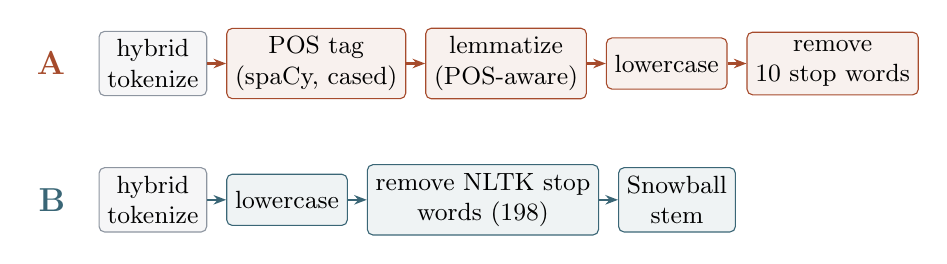
\begin{tikzpicture}[font=\small, node distance=2.4mm,
  st/.style={draw, rounded corners=2pt, minimum height=6.5mm, align=center, inner sep=3pt},
  arr/.style={-{Stealth[length=1.6mm]}, thick}]
  \node[st, draw=ink!50, fill=ink!4] (ta) {hybrid\\tokenize};
  \node[st, right=of ta, draw=pipeA, fill=pipeA!8] (a1) {POS tag\\(spaCy, cased)};
  \node[st, right=of a1, draw=pipeA, fill=pipeA!8] (a2) {lemmatize\\(POS-aware)};
  \node[st, right=of a2, draw=pipeA, fill=pipeA!8] (a3) {lowercase};
  \node[st, right=of a3, draw=pipeA, fill=pipeA!8] (a4) {remove\\10 stop words};
  \foreach \a/\b in {ta/a1,a1/a2,a2/a3,a3/a4} \draw[arr, pipeA] (\a) -- (\b);
  \node[st, below=9mm of ta, draw=ink!50, fill=ink!4] (tb) {hybrid\\tokenize};
  \node[st, right=of tb, draw=pipeB, fill=pipeB!8] (b1) {lowercase};
  \node[st, right=of b1, draw=pipeB, fill=pipeB!8] (b2) {remove NLTK stop\\words (198)};
  \node[st, right=of b2, draw=pipeB, fill=pipeB!8] (b3) {Snowball\\stem};
  \foreach \a/\b in {tb/b1,b1/b2,b2/b3} \draw[arr, pipeB] (\a) -- (\b);
  \node[left=3mm of ta, pipeA, font=\bfseries\large] {A};
  \node[left=3mm of tb, pipeB, font=\bfseries\large] {B};
\end{tikzpicture}
\vskip1em
\begin{columns}[T]
\begin{column}{.47\textwidth}
\begin{block}{\textcolor{white}{A: annotate first (linguist)}}
Tag while capitals and context still exist, then reduce to dictionary forms.\\
\emph{Bet: careful analysis keeps names and meanings intact.}
\end{block}
\end{column}
\begin{column}{.47\textwidth}
\begin{block}{\textcolor{white}{B: normalise first (IR engineer)}}
Lowercase at once, drop all common words, chop to stems \parencite{manning2008iir}.\\
\emph{Bet: aggressive merging, more matches, smaller index.}
\end{block}
\end{column}
\end{columns}
\end{frame}

\begin{frame}{Why each step sits where it does}{Every process: dependency, and what breaks if it moves}
\begin{table}
\footnotesize
\begin{tabular}{p{.16\textwidth}p{.19\textwidth}p{.22\textwidth}p{.31\textwidth}}
\toprule
Process & Position & Depends on & If moved \\
\midrule
Cleaning & first & raw text & artefacts (\texttt{[12]}, \emph{é}) become tokens \\
Name merging & inside tokenization & original case, stop words present & after stop removal or stemming, names stop matching the lexicon \\
POS tagging (\A) & before lowercasing & case, context & \emph{Halo} loses its proper-noun clue and gets lemmatized \\
Lemmatization (\A) & after tagging & POS tags & without POS, WordNet under-merges (UI 0.62--0.87) \\
Stop words (\B) & before stemming & lowercase & stem-first leaks \texttt{thi}, \texttt{wa}, \texttt{ha} \\
Query processing & same as documents & the pipeline & query terms would not match index terms \\
\bottomrule
\end{tabular}
\end{table}
\end{frame}

\begin{frame}{One sentence through both pipelines}{\emph{``The Legend of Zelda: Majora's Mask was released for the Nintendo 64 in 2000 and players were praising it.''}}
\begin{table}
\footnotesize
\begin{tabular}{llll}
\toprule
Token & POS & \A{} term & \B{} term \\
\midrule
The\_Legend\_of\_Zelda & NN & the\_legend\_of\_zelda & the\_legend\_of\_zelda \\
Nintendo\_64 & NNP & nintendo\_64 & nintendo\_64 \\
was & VBD & \pA{be} & \muted{(removed)} \\
released & VBN & \pA{release} & \pB{releas} \\
players & NNS & player & player \\
praising & VBG & \pA{praise} & \pB{prais} \\
\bottomrule
\end{tabular}
\caption{\texttt{pipeline\_trace\_example.csv} (abridged)}
\end{table}
\begin{itemize}
  \item \A{} keeps \alert{real words}; \B{} keeps fewer, truncated stems
  \item both protect \alert{names identically}: the tokenizer merged them before either pipeline started
\end{itemize}
\end{frame}

% =====================================================================
\section{Implement}
\roadmap{3}{3}{Build the indexer and the Boolean searcher, shared by both pipelines}

\begin{frame}[fragile]{The positional inverted index}{The data structure at the heart of the system}
\begin{columns}[T]
\begin{column}{.52\textwidth}
\textbf{term $\rightarrow$ document $\rightarrow$ positions}
\vskip0.3em
{\footnotesize
\begin{verbatim}
"game_boy": {"D01": [3893], "D03": [1978],
             "D05": [5237], ...}   12 docs
"metroid":  {"D01": [2160], "D05": [5808, 7090],
             "D08": [790, 1091, 1558], ...}
\end{verbatim}}
\begin{itemize}
  \item positions make \alert{phrase search} possible
  \item same idea as Lucene / Elasticsearch, without compression
\end{itemize}
\end{column}
\begin{column}{.44\textwidth}
\begin{table}
\small
\begin{tabular}{lrr}
\toprule
 & \A & \B \\
\midrule
Terms & 13,165 & 11,247 \\
Postings & 53,258 & 47,557 \\
Positions & 176,387 & 137,253 \\
In only 1 doc & 54\% & 53\% \\
\bottomrule
\end{tabular}
\caption{\texttt{index\_structure.csv}}
\end{table}
\muted{\small Zipf: most terms are rare and carry the information; terms in every document get an idf of 0.}
\end{column}
\end{columns}
\end{frame}

\begin{frame}{The searcher and the 12 test queries}{Boolean decides \emph{which} documents; ranking decides \emph{in what order}}
\begin{columns}[T]
\begin{column}{.44\textwidth}
\begin{enumerate}
  \item query runs through the \alert{same pipeline} as the documents
  \item AND = intersect, OR = union, NOT = subtract posting lists; phrases checked by position
  \item matches ranked by TF-IDF cosine, title matches $\times 2$
\end{enumerate}
\end{column}
\begin{column}{.53\textwidth}
\begin{table}
\scriptsize
\begin{tabular}{lll}
\toprule
& Query & Type \\
\midrule
Q01 & \texttt{Total War} & keyword (bigram) \\
Q03 & \texttt{Nintendo AND PlayStation} & AND \\
Q04 & \texttt{"Ash Ketchum" AND NOT Japanese} & NOT \\
Q06 & \texttt{Zelda AND (theme OR song)} & OR \\
Q07 & \texttt{"Tomb Raider"} & phrase \\
Q09 & \texttt{"Guitar Hero Live"} & phrase (trigram) \\
Q12 & \texttt{SNES OR "Super Nintendo \dots"} & OR \\
\bottomrule
\end{tabular}
\caption{7 of the 12 queries; every type covered}
\end{table}
\end{column}
\end{columns}
\end{frame}

% =====================================================================
\section{Compare \& Evaluate}
\roadmap{4}{5}{Predictions first, then the numbers}

\begin{frame}{What we predicted, before running anything}{Six preregistered hypotheses}
\begin{table}
\footnotesize
\begin{tabular}{llll}
\toprule
& Prediction & Evidence & Verdict \\
\midrule
H1 & \B{} has fewer tokens and a smaller vocabulary & 176,387 vs 137,253; 13,165 vs 11,247 & \textcolor{good}{\textbf{supported}} \\
H2 & \B{} has higher recall & R 0.796 vs 0.796 & no difference \\
H3 & \A{} has higher precision, esp.\ phrases & P 0.596 vs 0.596 & no difference \\
H4 & \B{} makes false phrase matches & 16 vs 28 docs (probe) & \textcolor{good}{\textbf{supported}}\textsuperscript{*} \\
H5 & \A{} preserves $\geq$5 pts more names & 1.000 vs 0.898 & \textcolor{good}{\textbf{supported}} \\
H6 & \A{} has more meaningful bigrams & 0.30 vs 1.00 & \textcolor{pipeA}{\textbf{rejected}} \\
\bottomrule
\end{tabular}
\caption{\texttt{hypotheses.csv}. \textsuperscript{*}exploratory: not testable on the 12 queries}
\end{table}
\muted{\small Reporting the predictions that failed is part of the result: H2, H3 and H6 did not hold.}
\end{frame}

\begin{frame}{Pipeline comparison}{Table H: the brief's required comparison}
\begin{columns}[T]
\begin{column}{.6\textwidth}
\begin{table}
\footnotesize
\begin{tabular}{lccc}
\toprule
Measure & \A & \B & Final (\A) \\
\midrule
Token count & 176,387 & 137,253 & 176,387 \\
Vocabulary size & 13,165 & 11,247 & 13,165 \\
Meaningful bigrams & 0.30 & 1.00 & 0.30 \\
Name preservation & \alert{1.000} & 0.898 & 1.000 \\
Precision (macro) & 0.596 & 0.596 & 0.596 \\
Recall (macro) & 0.805 & 0.805 & 0.805 \\
F1 (macro) & \alert{0.648} & \alert{0.648} & 0.648 \\
P@5 / P@10 & .583 / .367 & .583 / .367 & .583 / .367 \\
\bottomrule
\end{tabular}
\caption{\texttt{pipeline\_comparison.csv}}
\end{table}
\end{column}
\begin{column}{.36\textwidth}
\small
\begin{itemize}
  \item \B{} index \alert{29\% smaller}
  \item \A{} keeps \alert{all 128 names}; \B{} breaks 13 (\emph{Civilization} $\rightarrow$ \texttt{civil})
  \item \textbf{identical search results} on all 12 queries
  \item the bigram test favours \B{} by construction (it checks the stop list \B{} removed)
\end{itemize}
\end{column}
\end{columns}
\end{frame}

\begin{frame}{Retrieval performance}{Why accuracy is the wrong metric for search}
\begin{columns}[T]
\begin{column}{.48\textwidth}
\begin{table}
\footnotesize
\begin{tabular}{lccc}
\toprule
Query type & P & R & F1 \\
\midrule
AND & 0.722 & 0.963 & \alert{0.798} \\
phrase & 0.738 & 0.833 & 0.778 \\
keyword & 0.636 & 0.875 & 0.643 \\
OR & 0.400 & 0.929 & 0.556 \\
NOT & 0.350 & 0.333 & \textcolor{pipeA}{0.325} \\
\midrule
\textbf{All 12} & 0.596 & 0.805 & 0.648 \\
\bottomrule
\end{tabular}
\caption{\texttt{retrieval\_by\_query\_type.csv} (same for \A{} and \B)}
\end{table}
\end{column}
\begin{column}{.48\textwidth}
\begin{table}
\footnotesize
\begin{tabular}{lcc}
\toprule
 & relevant & not relevant \\
\midrule
retrieved & TP 48 & FP 56 \\
not retrieved & FN 9 & TN 523 \\
\bottomrule
\end{tabular}
\caption{Confusion matrix, all 636 pairs}
\end{table}
\begin{alertblock}{Accuracy misleads}
\small Our searcher: accuracy \textbf{0.898}. Returning \emph{nothing}: \textbf{0.910}.
Most documents are irrelevant to any query, so we report precision and recall.
\end{alertblock}
\end{column}
\end{columns}
\end{frame}

\begin{frame}{Where the searcher goes wrong}{Every error classified: 9 misses, 56 false hits, same for both pipelines}
\begin{columns}[T]
\begin{column}{.5\textwidth}
\begin{table}
\small
\begin{tabular}{lcc}
\toprule
Cause & FN & FP \\
\midrule
Passing mention & 0 & 54 \\
Query formulation & 6 & 0 \\
Wrong relevance label & 3 & 2 \\
\textbf{Any preprocessing step} & \alert{0} & \alert{0} \\
\bottomrule
\end{tabular}
\caption{\texttt{error\_analysis.csv}}
\end{table}
\end{column}
\begin{column}{.47\textwidth}
\begin{itemize}
  \item \textbf{NOT throws away answers}: \texttt{"Ash Ketchum" AND NOT Japanese} loses the \emph{Ash Ketchum} article, which mentions his Japanese voice actress
  \item \textbf{Passing mentions}: \texttt{Metroid} returns 11 documents; the 3 relevant ones rank 1--3, the rest are console histories
\end{itemize}
\end{column}
\end{columns}
\vskip0.2em
\muted{\small No error comes from tokenization, stemming, lemmas, stop words or NER, which is why \A{} and \B{} tie.}
\end{frame}

% =====================================================================
\section{Justify}
\roadmap{6}{6}{Apply the rule fixed in advance, and explain what the numbers mean}

\begin{frame}{Choosing the final pipeline}{A rule fixed in advance, applied in order}
\begin{enumerate}
  \item \textbf{F1 gap $\geq 0.05$?} \quad \A{} 0.648, \B{} 0.648, gap 0.000 \(\rightarrow\) \muted{does not decide}
  \item \textbf{Domain-term preservation gap $\geq 0.05$?} \quad \A{} 1.000, \B{} 0.898, gap \alert{0.102} \(\rightarrow\) \textbf{decides}
  \item \muted{Meaningful-bigram rate: not reached}
\end{enumerate}
\vskip0.6em
\begin{exampleblock}{Final pipeline: A (annotate first, lemmas)}
\A{} is \emph{not} chosen because it searches better; on this corpus it does not.
It is chosen because, when both find the same documents, \A's index represents the domain's names faithfully:
the term dictionary, postings and n-grams a person reads are real words and intact names.
\end{exampleblock}
\vskip0.3em
\muted{\small The cost of \A: a 29\% larger index and slower indexing (spaCy tagger). Query time: a few ms for both, within run-to-run noise.}
\end{frame}

\begin{frame}{An earlier run chose B: what we learned}{One oddly worded query decided a whole comparison}
\begin{columns}[T]
\begin{column}{.5\textwidth}
\begin{itemize}
  \item first run: queries worded \alert{automatically} from each question's first content words
  \item \emph{``Was there a Sonic game on the Sega Genesis?''} became \texttt{"there Sonic game"}
  \item \B{} drops \emph{there} as a stop word and finds the answers; \A{} keeps it and finds nothing
\end{itemize}
\end{column}
\begin{column}{.46\textwidth}
\begin{table}
\small
\begin{tabular}{lcc}
\toprule
F1 (automatic wording) & \A & \B \\
\midrule
all 12 queries & 0.183 & \alert{0.237} \\
without Q02 & \alert{0.200} & 0.176 \\
\bottomrule
\end{tabular}
\caption{reproduced exactly, 12/12 queries}
\end{table}
\end{column}
\end{columns}
\vskip0.4em
\begin{block}{What we did about it}
Queries rewritten by hand under a stated rule, \emph{before} any new result existed; the amendment is dated and both runs are reported.
\textbf{Finding:} differences between the pipelines come from stop words and inflections in the \emph{query wording}, not from how they handle domain content.
\end{block}
\end{frame}

\begin{frame}{Why the pipelines agree, and the design lesson}
\begin{columns}[T]
\begin{column}{.5\textwidth}
\textbf{Why they tie}
\begin{itemize}
  \item both share the component that matters most: the \alert{name-merging tokenizer}
  \item our queries are about names; \texttt{tomb\_raider} is never stemmed or lemmatized
  \item \A{} and \B{} differ on verb endings and function words, which the queries never touch
\end{itemize}
\end{column}
\begin{column}{.46\textwidth}
\begin{exampleblock}{Design lesson}
On an entity-heavy domain, the decisive preprocessing choice is the \textbf{domain-aware tokenizer and lexicon}, not stemming vs lemmatization.
\end{exampleblock}
\muted{\small Consistent with \textcite{brin1998anatomy}, who launched without stemming. Exploratory: no pipeline was run without name merging.}
\end{column}
\end{columns}
\end{frame}

% =====================================================================
\section{Demonstration}

\begin{frame}{The GUI: a working searcher with an X-ray}{9 tabs covering all 15 required functions}
\begin{columns}[T]
\begin{column}{.38\textwidth}
\footnotesize
\begin{itemize}
  \item \textbf{Search}: Boolean query, type, pipeline; ranked results, time, P / R / F1
  \item \textbf{Compare A vs B}: side by side, with a diff
  \item \textbf{Pipeline trace}: any sentence, stage by stage, timed
  \item \textbf{Corpus}, \textbf{Tokenization}, \textbf{POS \& NER}, \textbf{N-grams}
  \item \textbf{Index}: postings with positions and context
  \item \textbf{Evaluation}: the decision and every number
\end{itemize}
\muted{\scriptsize Every button calls the same pipelines and index as the report. Right: Search on Q03 with timing, precision, recall and the judged-relevant column.}
\end{column}
\begin{column}{.6\textwidth}
\begin{figure}
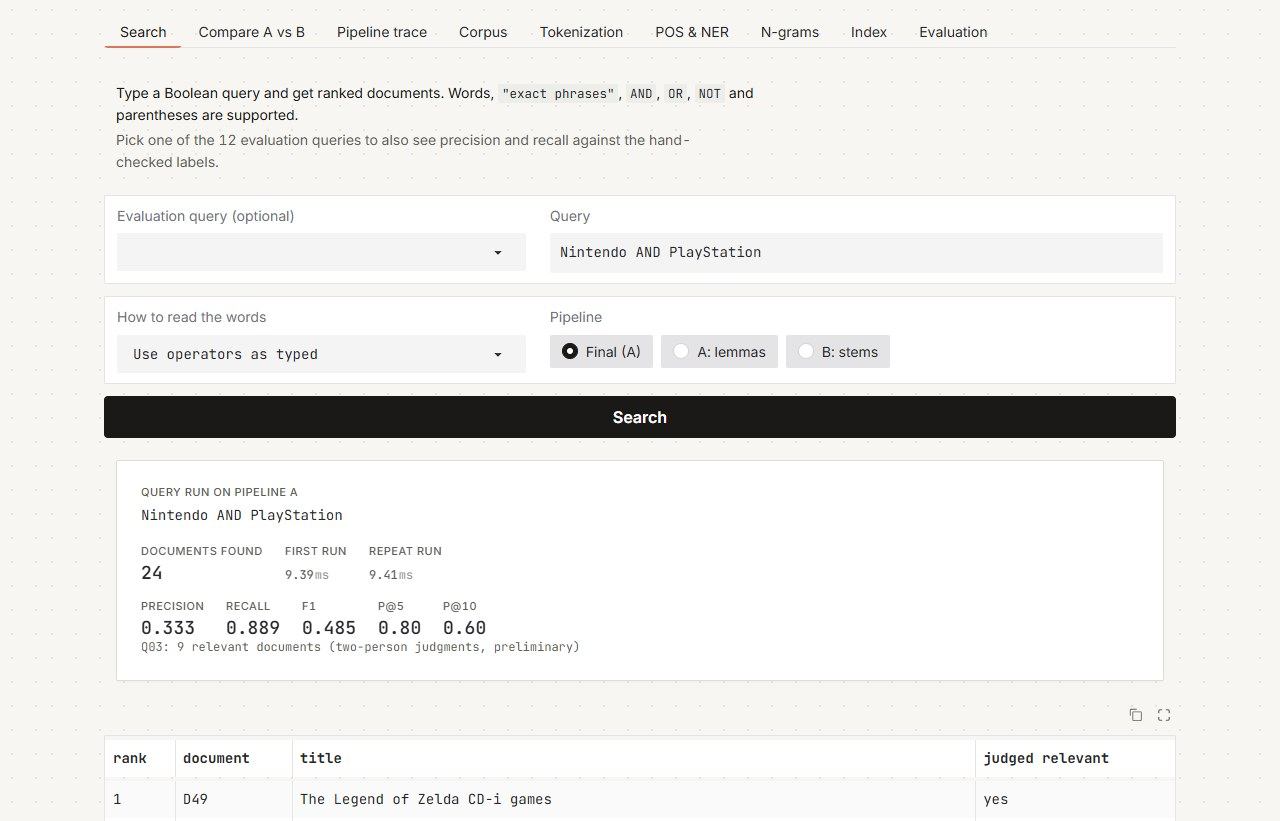
\includegraphics[width=\textwidth,height=.66\textheight,keepaspectratio]{img/gui_search.jpg}
\end{figure}
\end{column}
\end{columns}
\end{frame}

% =====================================================================
\section{Conclusion}

\begin{frame}{Limitations and next steps}
\begin{columns}[T]
\begin{column}{.49\textwidth}
\textbf{Limitations}
\begin{itemize}
  \item relevance labels: 2 reviewers, no agreement measure, $\geq 5$ labels look wrong \parencite{voorhees2000variations}
  \item 12 queries: too few for significance tests
  \item corpus built around its queries: absolute scores optimistic, A vs B unaffected
  \item lexicon of 128 names: unknown games still split
\end{itemize}
\end{column}
\begin{column}{.47\textwidth}
\textbf{Next steps}
\begin{itemize}
  \item blind relevance judging, more annotators
  \item 72 eligible questions; wordy queries to separate H2--H4
  \item one-component-at-a-time ablation with a paired test
  \item grow the lexicon from frequent n-grams (\emph{smash bros}); BM25 ranking
  \item a small knowledge graph from NER output
\end{itemize}
\end{column}
\end{columns}
\end{frame}

\begin{frame}{Conclusion}
\begin{enumerate}
  \item \textbf{The tokenizer matters most}: only a domain-aware tokenizer keeps names intact (91/91 vs 0/91).
  \item \textbf{Order is visible}: stem before stop-word removal and \texttt{thi}, \texttt{wa}, \texttt{ha} leak; tag before lowercasing or proper nouns get lemmatized.
  \item \textbf{General models miss the domain}: an EntityRuler lifts NER F1 from 0.563 to 0.744.
  \item \textbf{Both pipelines search identically} (P 0.596, R 0.805, F1 0.648); the preregistered rule selects \alert{Pipeline A} on name preservation.
  \item \textbf{Accuracy misleads}: 0.898 for our searcher, 0.910 for returning nothing.
\end{enumerate}
\vskip0.5em
\muted{\small All search results are preliminary until the relevance labels are re-judged by more annotators.}
\end{frame}

\section{References}
\begin{frame}[t, allowframebreaks]{\bibname}
\nocite{*}
\footnotesize
\printbibliography[heading=none]
\end{frame}

\begin{frame}[plain]
\vfill
\centerline{\Large\bfseries\color{ink}Thank You for Your Attention!}
\vskip0.6em
\centerline{\color{muted}Questions? \quad The GUI is ready for a live demo.}
\vfill\vfill
\end{frame}

\end{document}
